\label{pattern_mining}
In this section, we will detail our experiment using the \textbf{FP-Growth} algorithm to extract frequent itemsets and association rules. The most useful rules were then exploited to classify some relevant \textit{titleTypes}.

Preprocessing was required to turn the dataset into a list of transactions, with each record representing a transaction containing one item for each feature value associated with that record.
For multilabel variables \textit{genres} and \textit{CountryOfOrigin}, we created as many items as the values expressed in each record.
We augmented transactions representing titles produced in at least one country not in the top four (US, UK, FR, JP) adding the item \texttt{country\_Other} to the transaction, but also kept the specific countries in the transaction, in order to be able to detect possible patterns associated both with titles produced in a specific country and with titles produced in any less represented country.
Numeric variables were discretized into quartile-based bins, and, to allow interpretability, the name of the variables was appended to their values.
%\begin{table}[ht]
%\centering
%\resizebox{\columnwidth}{!}{%
%\begin{tabular}{|l|c|c|c|c|}
%\hline
%\textbf{Variable} & \textbf{Bin 1} & \textbf{Bin 2} & \textbf{Bin 3} & \textbf{Bin 4} \\
%\hline
%startYear & [1878, 1978] & (1978, 1997] & (1997, 2013] & (2013, 2024] \\
%runMins. & [0, 29] & (29, 50] & (50, 90] & (90, 3000] \\
%nVotes* & [1.792, 2.773] & (2.733, 3.611] & (3.611, 5.007] & (5.007, 13.782] \\
%totImgs* & [0, 0.693] & (0.693, 1.946] & (1.946, 8.162] & -- \\
%totCreds* & [0, 2.833] & (2.833, 3.555] & (3.555, 4.19] & (4.19, 9.66] \\
%numRegs* & (0.692, 1.386] & (1.386, 4.248] & -- & -- \\
%critRevRat & [0, 0.227] & (0.227, 1] & -- & -- \\
%\hline
%\end{tabular}
%}
%\caption{Bin intervals for each binned variable (*: log-transformed).}
%\label{tab:bin-intervals}
%\end{table}
\subsection{Frequent Itemsets Extraction}
We kept the minimum number of items in the itemsets (\textit{zmin}) fixed to two, as 2-itemsets could already be interesting. Fig. \ref{fig:max_closed_itemsets.png} shows the number of closed and maximal frequent itemsets extracted for different \textit{minsup} values, ranging from 2\% to 30\%. The number of itemsets drops quickly, and after 25\% the two groups seem to start converging to lower values (< 250). We also looked at the maximal frequent itemsets containing our target variable, \textit{titleType} (Fig. \ref{fig:max_itemsets_titleType.png}): there are none for the minority classes tvShort, videoGame, tvMiniSeries, tvSpecial, and we start losing more classes from \textit{minsup} > 4\%.

\begin{figure}
    \centering
    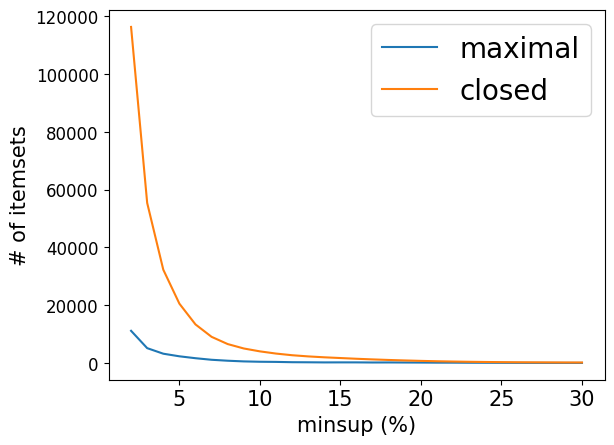
\includegraphics[width=0.8\columnwidth]{../results/images/max_closed_itemsets.png}
    \caption{N. of closed and maximal frequent itemsets for different \textit{minsup} values.}
    \label{fig:max_closed_itemsets.png}
\end{figure}

\begin{figure}
    \centering
    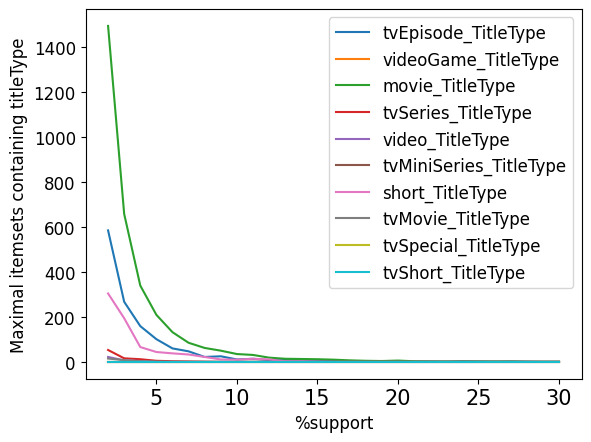
\includegraphics[width=0.8\columnwidth]{../results/images/max_itemsets_titleType.png}
    \caption{N. of maximal frequent itemsets containing \textit{titleType}for different \textit{minsup} values.}
    \label{fig:max_itemsets_titleType.png}
\end{figure}

After testing different \textit{minsup} values, we chose 30\%, as we got some interesting maximal itemsets, rather than just a combination of the most frequent values for the different features. At this threshold, the frequent itemsets are 174 and they are all closed, while the maximal itemsets are only 26. In Table \ref{tab:maximal_itemsets} are reported some of the most interesting maximal itemsets, among the top 10 with the highest support.
The first one captures a dependency we expect: a movie doesn't have episodes. This is similarly captured by the 7th, as the reported runtime is typical of movies and tv episodes. The 4th one represents many foreign titles, made in just one foreign country, while the 6th captures dramatic stand-alone titles from a single country: it can well describe telenovela episodes, or lower budget dramatic movies (as they are made in a single country).
\begin{table}
\small
%\setlength{\tabcolsep}{4pt}
\renewcommand{\arraystretch}{0.9}
\centering
\begin{tabular}{|>{\centering\arraybackslash}p{0.7cm}|>{\raggedleft\arraybackslash}p{4.1cm}|c|}
\hline
\textbf{Rank} & \textbf{Maximal Itemset} & \textbf{Sup} \\
\hline
1 & (movie\_TitleType, NoEpisodes) & 33.686 \\
\hline
4 & (country\_Other, NoVideos, OneCountryofOrigin) & 32.481 \\
\hline
6 & (genre\_Drama, NoEpisodes, OneCountryofOrigin) & 31.514 \\
\hline
7 & ((50.0, 90.0]\_RuntimeMin, NoEpisodes) & 31.471 \\
\hline
\end{tabular}
\caption{Selected top maximal itemsets for \textit{minsup}=30.}
\label{tab:maximal_itemsets}
\end{table}

\subsection{Association Rule Extraction}
The heatmap in Fig. \ref{fig:heatmap_association_rules.png} shows the number of association rules extracted by the FP-Growth algorithm for different \textit{minsup} and confidence (\textit{minconf}) thresholds. It is evident that the number of rules drops quickly as the \textit{minsup} increases, while it is less affected by \textit{minconf}. Therefore, we first kept a fixed low value of confidence (65\%) and experimented with different values of \textit{minsup}, increasing it by small increments. Once we found a value yielding an interesting list of rules, we increased the confidence threshold. We reached 80\% \textit{minconf} before losing interesting rules. The final hyperparameters are: \textit{zmin}=2, \textit{minsup}=9\% and \textit{minconf}=80\%.
\begin{figure}
    \centering
    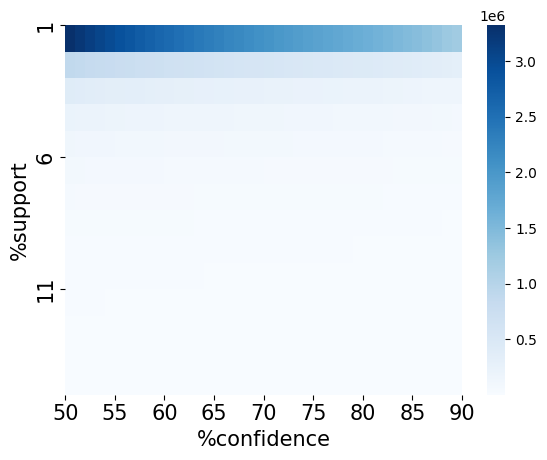
\includegraphics[width=0.8\columnwidth]{../results/images/heatmap_association_rules.png}
    \caption{N. of association rules extracted for different \textit{minsup} and \textit{minconf} values.}
    \label{fig:heatmap_association_rules.png}
\end{figure}

The total number of rules extracted is 16466. The histograms in Fig. \ref{fig:rules_conf_lift.png} show the rules' confidence and lift distributions. While most rules exhibit a confidence greater than 0.87, the vast majority are weak, with a lift below 1.
\begin{figure}
    \centering
    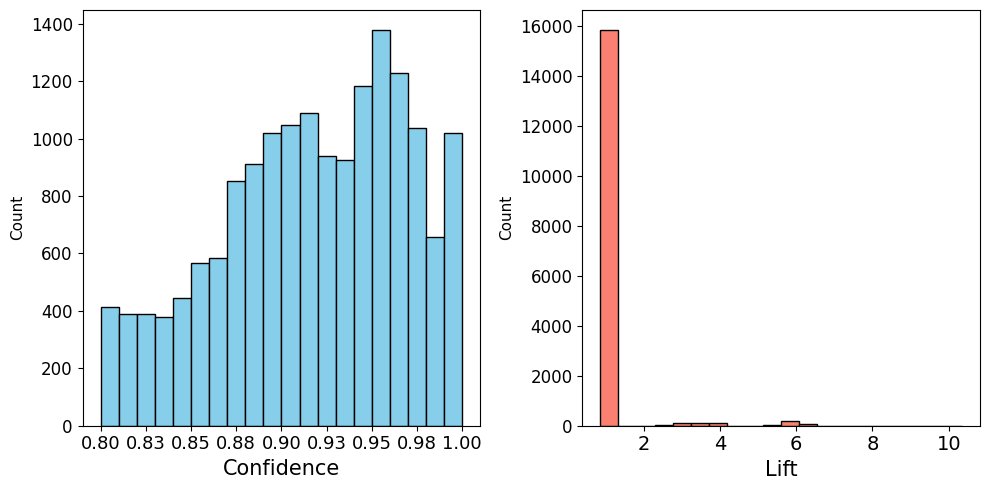
\includegraphics[width=\columnwidth]{../results/images/rules_conf_lift.png}
    \caption{Histograms of rules' confidence and lift.}
    \label{fig:rules_conf_lift.png}
\end{figure}

The 30 rules with the highest lift all contain a \textit{titleType} either in the antecedent or consequent; a selection is reported in Table \ref{tab:top_association_rules}. In particular, the two top rules have captured the fact that tvSeries have episodes, while the rest have captured the redundancy of the information about shorts, present in both \textit{genres} and \textit{titleType}. In particular, rules having \textit{short\_titleType} as consequent are all associated with both \textit{genre\_Short} and the lowest value for \textit{runtimeMinutes}, [0, 29].

\begin{table}
    \small  % Shrinks font size for table
    \setlength{\tabcolsep}{3pt}  % Reduces column padding
    %\renewcommand{\arraystretch}{0}  % Reduces row height
    \centering
    \begin{tabular}{|p{3cm}|p{1.4cm}|c|c|c|}
    \hline
    \textbf{Antecedent} & \textbf{Conseq.} & \textbf{\%sup} & \textbf{conf} & \textbf{lift} \\
    \hline
    (HasEpisodes,\newline OneCountryofOrigin) & tvSeries\newline \_TitleType & 7.89 & 0.866 & 10.35 \\
    \hline
    (HasEpisodes) & tvSeries\newline \_TitleType & 8.37 & 0.860 & 10.28 \\
    \hline
    (short\_TitleType,\newline {[}0, 0.693{]}\_Total-\newline Images, NoEpisodes) & genre\newline\_Short & 8.48 & 0.931 & 6.21 \\
    \hline
    (genre\_Short,\newline {[}0, 29{]}\_RuntimeMin, \newline(0.692, 1.386]\_Num-\newline Regions, NoEpisodes,\newline OneCountryofOrigin) & short\newline \_TitleType & 11.33 & 0.933 & 6.20 \\
    \hline
    (short\_TitleType,\newline {[}0, 2.833{]}\_TotalCredits, NoEpisodes) & genre\newline\_Short & 8.58 & 0.928 & 6.19 \\
    \hline
    \end{tabular}
    \caption{Selected top association rules by lift.}
    \label{tab:top_association_rules}
\end{table}

\subsection{Classification: \textit{titleType}}
Out of the extracted rules, 245 have a \textit{titleType} in the consequent: 144 have short, 89 have tvEpisode, 10 have movie, and two have tvSeries.
For each of these four \textit{titleType} classes, we implemented the rule with the highest support for a task of multiclass classification, for the sake of which the remaining classes were aggregated to 'Other'. We favored the rules with the highest support because they are more general and include the most important items in the antecedent; nevertheless, we made sure that their lift was higher than 1. The selected rules are reported in Table \ref{tab:association_rules_titleType}.

\begin{table}
    \small  % Shrinks font size for table
    \setlength{\tabcolsep}{4pt}  % Reduces column padding
    \renewcommand{\arraystretch}{1}  % Reduces row height
    \centering
    \begin{tabular}{|p{2.4cm}|p{1.4cm}|c|c|c|}
    \hline
    \textbf{Antecedent} & \textbf{Conseq.} & \textbf{\%sup} & \textbf{conf} & \textbf{lift} \\
    \hline
    (genre\_Short, NoEpisodes) & short\newline \_TitleType & 13.42 & 0.900 & 5.980 \\
    \hline
    ((29.0, 50.0]\_\newline RuntimeMin, NoEpisodes) & tvEpisode\newline \_TitleType & 16.57 & 0.873 & 3.054 \\
    \hline
    ((90.0, 3000.0]\_\newline RuntimeMin, NoEpisodes)	 & movie\newline \_TitleType & 12.85 & 0.824 & 2.446 \\
    \hline
    (HasEpisodes) & tvSeries\newline \_TitleType & 8.37 & 0.860 & 10.276 \\
    \hline
    \end{tabular}
    \caption{Association rules for \textit{titleType} classification.}
    \label{tab:association_rules_titleType}
\end{table}

Our simple rule-based classifier  achieved an accuracy of 60\% and a macro F1 score of 67.5\% on the test set, outperforming our baseline model, a stratified dummy classifier trained on the training set, across all metrics for all classes (accuracy: 0.25, macro F1: 0.20).

The confusion matrix in Fig. \ref{fig:heatmap_classification_rules_tts.png} allows us to understand what types of mistakes the classifier made and how the 'Other' classes were classified.
The information about having episodes was enough to achieve perfect recall for tvSeries, but of course all tvMiniSeries were also classified as such. The same happens for tvShorts, all classified as shorts – the same had happened for our other classifiers. The information about \textit{runtimeMinutes} has lead to some misclassification, as the binning is quite coarse-grained; this explains the lower recall for tvEpisodes and, especially, for movies: there's plenty of movies with a runtime < 90 minutes. All of our classification models have yielded better performances for these two classes: the information carried by the other features proved to be useful.

\begin{figure}
    \centering
    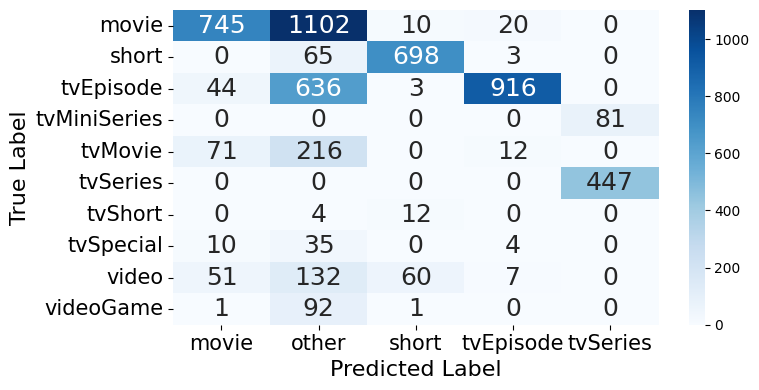
\includegraphics[width=\columnwidth]{../results/images/heatmap_classification_rules_tts.png}
    \caption{Confusion Matrix for rule-based classifier (10 True × 5 Predicted).}
    \label{fig:heatmap_classification_rules_tts.png}
\end{figure}
In conclusion, the selected association rules leveraged runtime, the information about serialized format, and the explicit information about shorts: these were exactly the top three most important features for our DT classifier. Using significantly less information than our classifiers, they were able to yield satisfactory results for these relevant classes.